\section{Classificazione di Hubble}\label{sec:classificazione-di-hubble}
Le galassie sono sistemi celesti auto-gravitanti composti da circa $10^3$ - $10^7$ stelle, ma anche da polvere, gas e materia oscura. Sono l'unico posto dell'Universo in cui possiamo trovare stelle, nello spazio interstellare NON sono presenti stelle isolate (a parte alcune nel mezzo inter-galattico degli ammassi di galassie e le prime stelle formatesi nell’Universo, Pop III?).
Una prima classificazione delle galassie può essere fatta in base alla loro morfologia, individuando tre classi principali:
\begin{itemize}
	\item a spirale;
	\item ellittiche (o \textit{early-tipe});
	\item irregolari e peculiari.
\end{itemize}

Una classificazione ulteriore delle galassie è data dalla cosiddetta \emph{classificazione di Hubble}, che è rappresentata
dal diagramma a forcella in figura~\ref{fig:classificazione-di-hubble}:
\begin{itemize}
	\item Le galassie ellittiche sono classificate in base alla loro ellitticità, con un indice crescente da E0 a E7 (E0 corrisponde a una forma circolare, mentre E7 indica le galassie più ellittiche).
	\item Le galassie a spirale sono distinte in: spirali normali (S) e le spirali barrate (SB) e per entrambe ci sono sotto classificazioni: a, b, c. A seconda della lettera cambia il grado di avvolgimento dei bracci a spirale (Sa e SBa hanno bracci di spirale più avvolti intorno al nucleo rispetto a quelle Sc e SBc). Le galassie indicate con S0, anche dette lenticolari, sono galassie a disco che non mostrano evidenza di bracci nel disco.
	\item Come possiamo vedere le galassie irregolari e peculiari non sono incluse nella classificazione di Hubble.
\end{itemize}

\begin{figure}
	\centering
	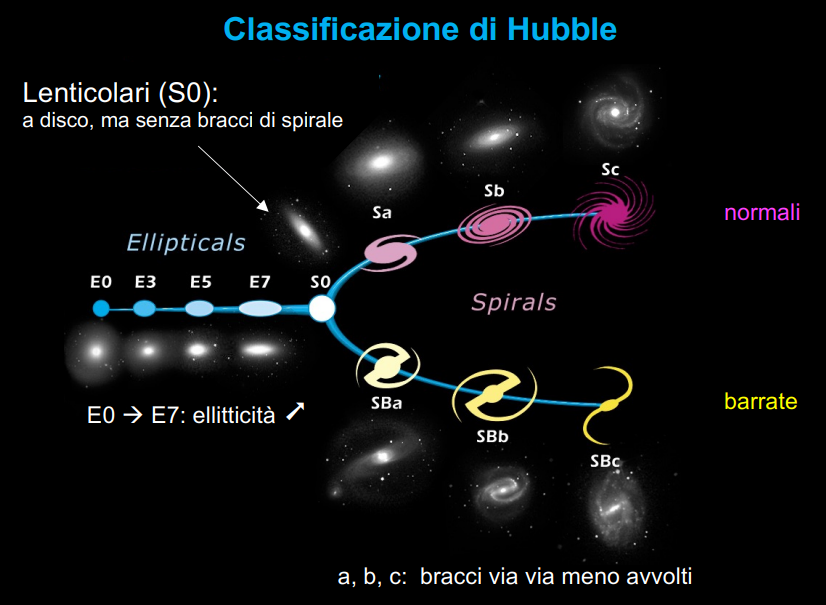
\includegraphics[width=0.6\textwidth]{immagini/classificazione-di-hubble.png}
	\caption{Classificazione di Hubble}
	\label{fig:classificazione-di-hubble}
\end{figure}

La cosa più importante da tenere in considerazione quando si osserva il diagramma a forcella della classificazione di Hubble è che \emph{non si tratta di una sequenza evolutiva!} Non dobbiamo mai pensare che questo diagramma indichi che le galassie ellittiche evolvano verso galassie a spirale, è solo un modo per classificare il tipo di galassie esistenti.

\subsection{Galassie a spirale} Sono composte da dischi sottili con braccia a spirale e sono composte da stelle, gas e polvere con distribuzione non omogenea (le stelle sono organizzate lungo bracci a spirale). Al centro del disco c’è un rigonfiamento sferico chiamato bulge; attorno ad esso c’è un alone molto esteso quasi vuoto che presenta qualche ammasso globulare (alone costituito da molto meno materia rispetto al disco e al bulge). Nei bracci a spirale c’è formazione stellare in corso: ho stelle giovani, con età sotto 10 ml di anni e ricche di metalli (popolazione I), a causa della presenza di gas arricchiti dalle generazioni precedenti di stelle. Nel bulge e nell’alone non c’è formazione stellare in corso, quindi sono costituiti da stelle vecchie, con età sopra 12 mld di anni (popolazione II). Circa i 2/3 delle galassie a spirale sono spirali barrate, cioè oltre al bulge è presente una barra centrale ai cui estremi si diramano i bracci; anche la Via Lattea è una spirale barrata (SBc).

Una galassia a spirale è caratterizzata dalle seguenti caratteristiche generali:
\begin{itemize}
	\item \emph{MASSA:} $10^9 \si{\solarmass}$ fino a qualche $10^{11} \si{\solarmass}$ .
	\item \emph{DIMENSIONE (diametro):} da $\sim$ 5 kpc a varie decine di kpc.
	\item \emph{POPOLAZIONE STELLARE:} eterogenea (giovane e vecchia).
	\item \emph{COLORE:} soprattutto blu
	\item \emph{GAS, POLVERE:} soprattutto gas freddo; polvere nel disco, non nei bracci (dove c'è invece produzione stellare).
\end{itemize}

\subsection{Galassie ellittiche} Sono ellissoidi, costituiti essenzialmente da stelle di popolazione II, c’è pochissimo gas e pochissima polvere e ciò corrisponde al fatto che non c’è formazione stellare in corso (infatti le stelle si formano da gas freddo).

Una galassia ellittica è caratterizzata dalle seguenti caratteristiche generali:
\begin{itemize}
	\item \emph{MASSA:} da qualche $10^7 \si{\solarmass}$ (galassie ellittiche "nane") fino a $10^{12} - 10^{13} \si{\solarmass}$ (sono il tipo di galassia più massivo).
	\item \emph{DIMENSIONE (diametro):} da $\sim$ 1 kpc a varie decine di kpc.
	\item \emph{POPOLAZIONE STELLARE:} omogenea e vecchia ($5$ - $13$ Gyr).
	\item \emph{COLORE:} rosso
	\item \emph{GAS, POLVERE:} poco gas caldo (T $\sim$ $10^6/10^7$ K); no, poca polvere.
\end{itemize}

\begin{figure}
	\centering
	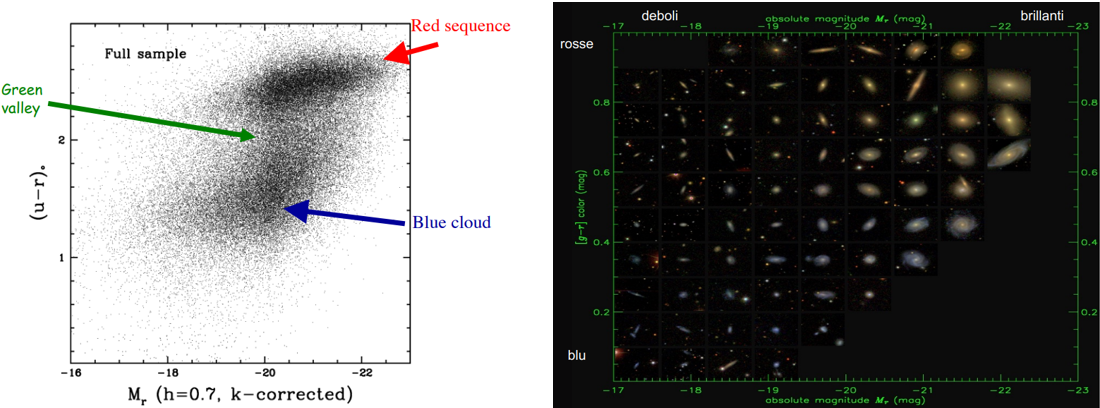
\includegraphics[width = \textwidth]{immagini/galassie-colore-magnitudine.png}
	\caption{In figura possiamo vedere una classificazione della magnitudine delle galassie in funzione del colore: notiamo come quelle che tendono più verso il rosso e sono più brillanti sono quelle di forma ellittiche. Le galassie a spirale risultano anch'esse abbastanza brillanti ma di colore blu (ci sono stelle più calde e più giovani).}
	\label{fig:galassie-colore-magnitudine}
\end{figure}

\subsection{Galassie irregolari e peculiari}
Sono galassie che non hanno una struttura riconoscibile, quindi non sono presenti bracci di spirale, disco o bulge riconoscibili; sono composte da un mix di gas e polvere, unito a stelle tendenzialmente di popolazione I. Molto spesso sono o galassie satelliti di altre galassie (quindi che ruotano attorno ad un'altra galassia) o sono in interazione con altre galassie e sono luoghi di intensa produzione stellare. Un esempio sono le due Nubi di Magellano (irregolari, perché hanno forma non ben definita), che sono galassie satellite della nostra galassia, ovvero risentono del potenziale della nostra galassia, e le Galassie Antenne (peculiari, perché hanno forma definita ma non canonica), che sono due galassie autointeragenti.

Una galassia irregolare o peculiare è caratterizzata dalle seguenti caratteristiche generali:

\begin{itemize}
	\item \emph{MASSA:} da qualche $10^7 \si{\solarmass}$ (galassie irregolari "nane") fino a $< 10^{10} \si{\solarmass}$.
	\item \emph{DIMENSIONE (diametro):} da $\sim$ 1 kpc a $\sim$ 10 kpc.
	\item \emph{POPOLAZIONE STELLARE:} soprattutto giovane.
	\item \emph{COLORE:} blu (per le "starburst" (quelle che formano stelle ad alto tasso) si ha colore rosso a causa della emissione della radiazione dalla polvere da cui si formano le stelle che riemette nel rosso come già visto in precedenza).
	\item \emph{GAS, POLVERE:} soprattutto gas freddo; polvere nel disco, non nei bracci (dove c'è invece produzione stellare).
\end{itemize}

\begin{figure}
	\centering
	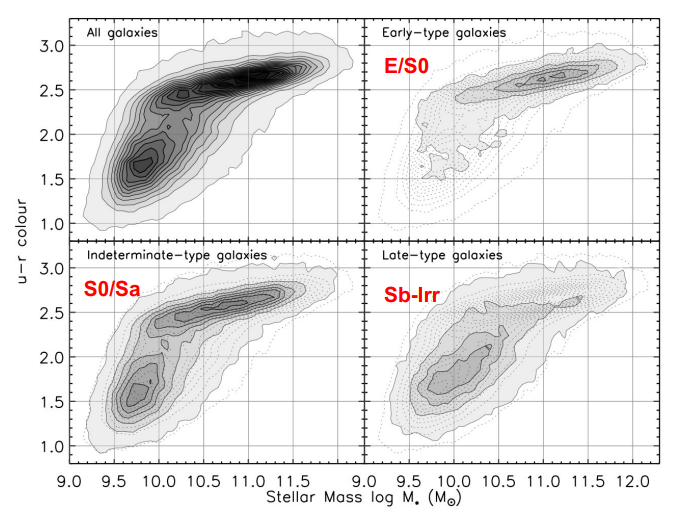
\includegraphics[width = 0.6 \textwidth ]{immagini/galassie-colore-massa-stellare.png}
	\caption{In figura possiamo vedere un grafico che confronta colore e massa delle galassie: come possiamo notare le galassie ellittiche sono le più massive e verso il rosso, le galassie a spirale sono in parte verso il rosso e in parte verso il blu (con masse confrontabili con quelle ellittiche), mentre quelle irregolari sono quasi tutte blu e con masse molto minori.}
	\label{fig:galassie-colore-massastellare}
\end{figure}
\subsection{Effetti ambientali}
Il nostro Universo non è riempito in modo omogeneo: sono presenti zone più dense (dette zone di cluster, dove avviene la formazione delle galassie), zone meno dense (dette ambienti di campo) e anche zone praticamente vuote, come si può vedere in figura~\ref{fig:non-omogeneo-universo}.

\begin{figure}
	\centering
	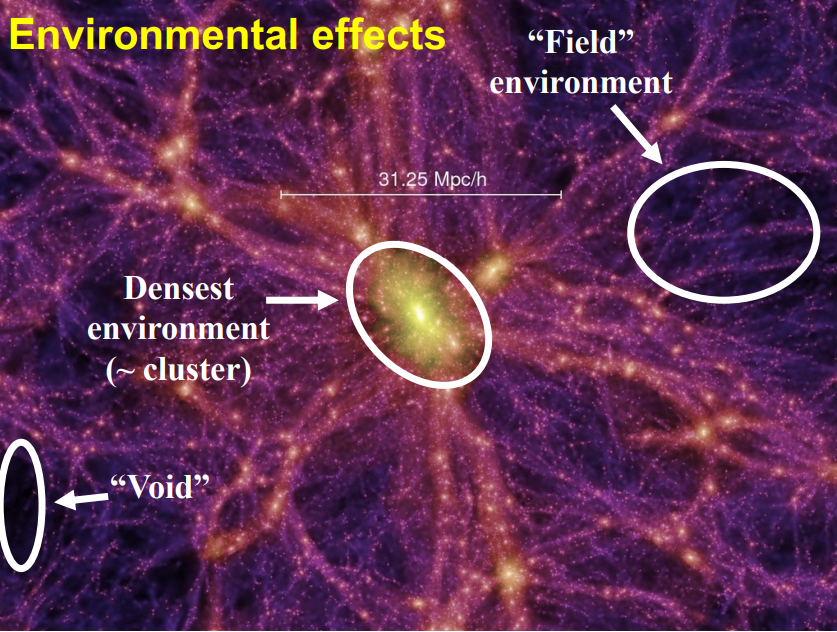
\includegraphics[width = 0.5\textwidth]{immagini/non-omogeneita-universo.png}
	\caption{In figura possiamo vedere rappresentate le tre tipologie di zone del nostro universo: cluster, ambienti di campo e spazio vuoto.}
	\label{fig:non-omogeneo-universo}
\end{figure}

Una domanda che sorge spontanea è: le diverse regioni di universo contengono stessi tipi morfologici di galassie oppure ci sono determinati tipi morfologici di galassie in diverse regioni di universo? Quello che è stato osservato è che negli ambienti di bassa densità (ossia gli ambienti di campo) c’è forte presenza di galassie spirali e irregolari (poche ellittiche e reticolari), mentre negli ambienti a più alta densità (ammassi di galassie) dominano le galassie reticolari e ellittiche (poche spirali), come è riassunto dal grafico in figura~\ref{fig:grafico-densità-morfologia}.

\begin{figure}[!htb]
	\centering
	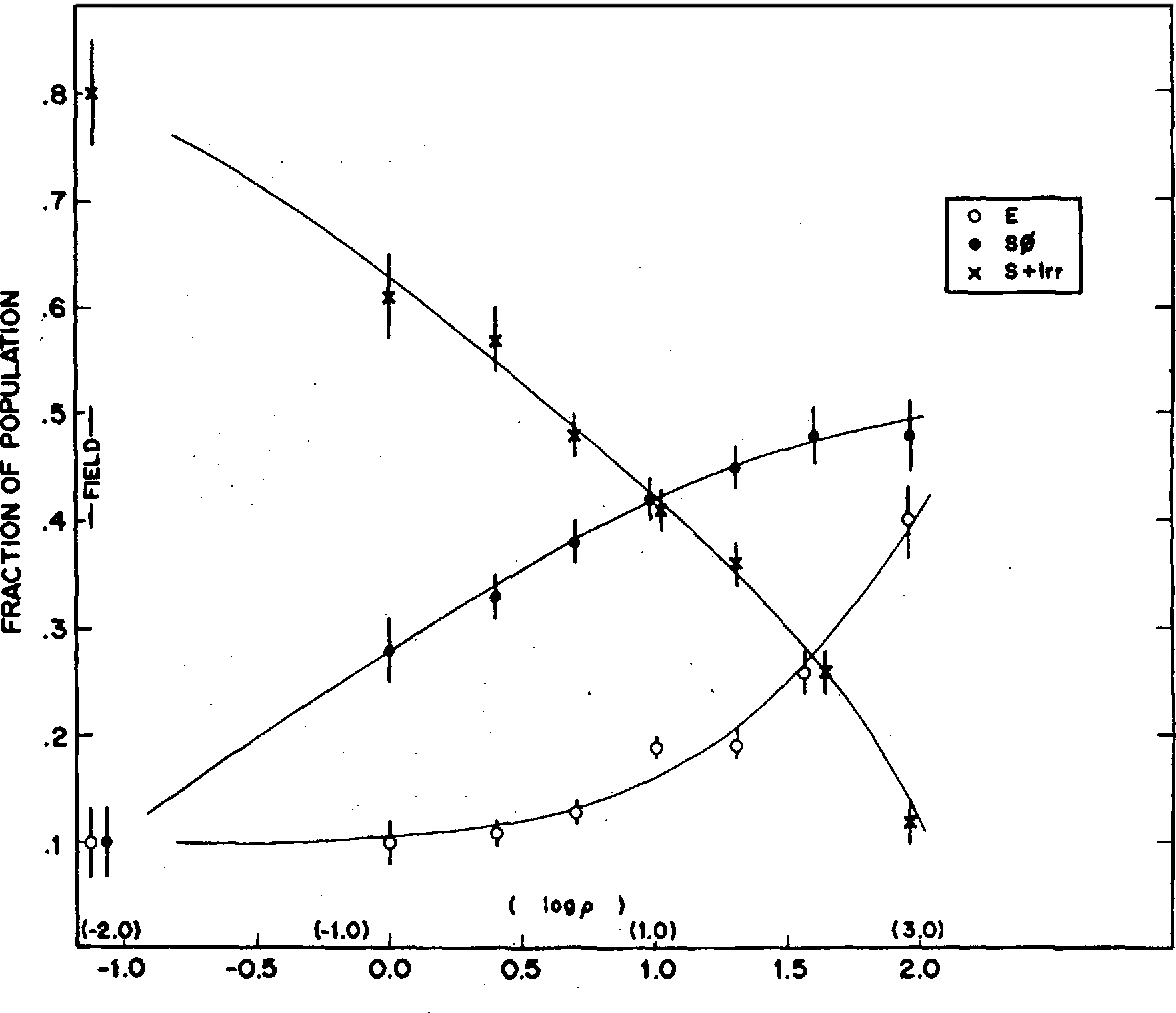
\includegraphics[width = 0.5\textwidth]{immagini/enviromental-density.png}
	\caption{Nel grafico viene evidenziato come a basse densità siano presenti soprattutto galassie a spirale; all'aumentare della densità queste diminuiscono ed aumentano le galassie ellittiche e reticolari.}
	\label{fig:grafico-densità-morfologia}
\end{figure}

Perché abbiamo questa distribuzione? Le galassie nascono in questa maniera oppure vengono trasformate dall’ambiente? È l’ambiente che riesce a modificare il tipo morfologico delle galassie oppure nascono direttamente in quel tipo in quella regione particolare? In realtà è una domanda ancora aperta, infatti si contrappongono due visioni del fenomeno differenti:

\begin{itemize}
	\item Da una parte infatti si ha il modello cosmologico di Cold Dark Matter (il migliore attualmente), che prevede che le regioni di alta densità sono anche le regioni più vecchie (formate prima) e infatti si ha che le galassie ellittiche sono più vecchie delle altre. Questo quindi sembrerebbe aver senso col dato sperimentale. Ma perché allora sono proprio le ellittiche a formarsi prima? Anche a questa domanda non c’è ancora risposta.
	\item D’altra parte, sappiamo che ci sono molti processi fisici che hanno impatto nella morfologia delle galassie (ad es. ram pressure stripping, galaxy harassment…), in particolare in ambienti densi ci sono fenomeni che possono distruggere le spirali; infatti a causa dell'alta densità i bracci formati dalla galassia vengono strappati da quelle accanto, trasformandole tutte in ellittiche. Tuttavia, pensiamo che le ellittiche si formino da merge di galassie, e la probabilità di merge è più bassa per cluster più massivi (perchè le velocità relative sono troppo alte per permettere una collisione e successiva fusione).
\end{itemize}

Quindi in entrambi gli scenari ci sono problemi e la questione è ancora aperta.